\title{Aula 8 - Circuitos e  Unidade Lógica e Aritmética}



\begin{frame}
    \titlepage
\end{frame}


\begin{frame}{Circuito Somador}

    \begin{figure}
        \centering

        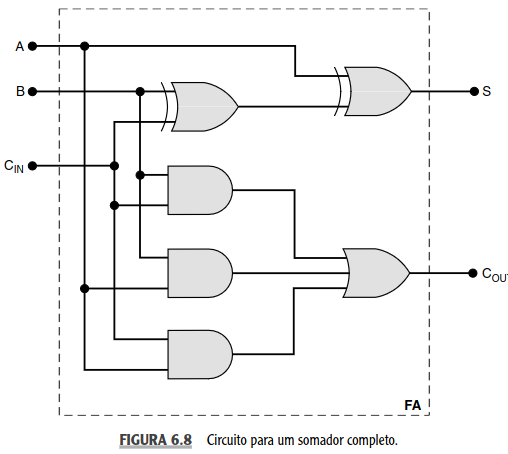
\includegraphics[width=0.7\textwidth]{Figuras/circuito-somador.png}

    \end{figure}

\end{frame}

\begin{frame}{Circuito Somador - Tabela verdade}

    \begin{figure}
        \centering

        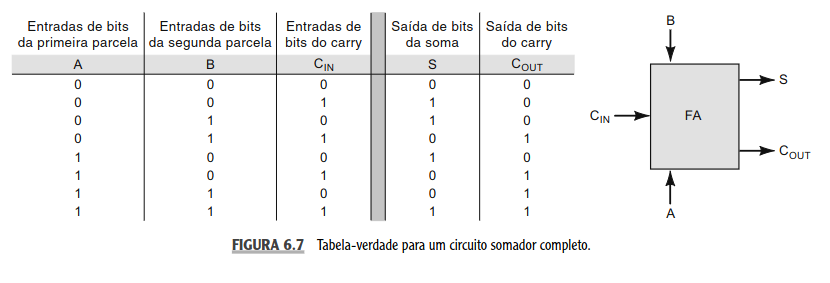
\includegraphics[width=\textwidth]{Figuras/tabela-verdade-somador.png}

    \end{figure}

\end{frame}


\begin{frame}{Unidade Lógica e aritmética}

    \begin{figure}
        \centering

        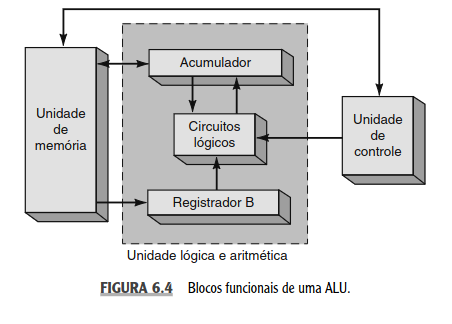
\includegraphics[width=\textwidth]{Figuras/ULA.png}

    \end{figure}

\end{frame}

\begin{frame}{A Unidade Lógica e Aritmética (ULA / ALU)}
    \begin{itemize}
        \item Todas as operações lógicas e aritméticas são realizadas na \textbf{unidade lógica e aritmética} (ALU) de um computador.
        \item \textbf{Objetivo principal:} Receber dados binários armazenados na memória e executar operações sobre eles, de acordo com instruções da unidade de controle.
    \end{itemize}

    \begin{block}{Estrutura Básica}
        Contém pelo menos dois registradores (\textbf{Registrador B} e \textbf{Acumulador}) e uma \textbf{lógica combinacional} que realiza as operações sobre os números armazenados neles.
    \end{block}
\end{frame}

\begin{frame}{Fluxo Típico de Operações}
    \begin{enumerate}
        \item \textbf{Instrução:} A unidade de controle decodifica a instrução indicando que um número de uma posição da memória deve ser somado ao \textbf{acumulador}.
        \item \textbf{Carga:} O número a ser somado é transferido da memória para o \textbf{registrador B}.
        \item \textbf{Processamento:} Os números de B e do acumulador são somados no circuito lógico. O resultado é enviado e \textbf{sobrescreve o acumulador}.
        \item \textbf{Destino:} O novo valor no acumulador pode ser mantido para sucessivas somas ou transferido de volta para a memória.
    \end{enumerate}

    \begin{alertblock}{O Papel do Acumulador}
        Ele \textit{"acumula"} os resultados dos passos intermediários de problemas aritméticos que implicam múltiplos passos, além do resultado final.
    \end{alertblock}
\end{frame}

\begin{frame}{As Quatro Operações na ALU}
    Apesar de a ALU ser baseada em circuitos somadores, ela consegue realizar todas as operações aritméticas fundamentais:

    \begin{itemize}
        \item \textbf{Soma:} Executada diretamente pelos circuitos somadores binários.
        \item \textbf{Subtração:} Realizada através da soma com o \textbf{complemento de dois} ($A - B = A + [B_{comp2}]$).
        \item \textbf{Multiplicação:} Implementada como uma sucessão de somas e deslocamentos de bits (\textit{shifts}).
        \item \textbf{Divisão:} Processada através de subtrações sucessivas e comparações.
    \end{itemize}

\end{frame}

\begin{frame}{Divisão por Subtrações Sucessivas (27 ÷ 5)}
    \textbf{Conceito:} A ALU realiza a divisão subtraindo o divisor do dividendo repetidamente até que o resultado seja menor que o divisor.

    \begin{columns}
        \begin{column}{0.5\textwidth}
            \begin{itemize}
                \item \textbf{Dividendo:} 27
                \item \textbf{Divisor:} 5
            \end{itemize}

            \begin{block}{Processo Iterativo}
                \begin{enumerate}
                    \item $27 - 5 = 22$ \quad (1ª subtração)
                    \item $22 - 5 = 17$ \quad (2ª subtração)
                    \item $17 - 5 = 12$ \quad (3ª subtração)
                    \item $12 - 5 = 7$ \quad \ (4ª subtração)
                    \item $7 - 5 = 2$ \quad \ (5ª subtração)
                \end{enumerate}
            \end{block}
        \end{column}

        \begin{column}{0.45\textwidth}
            \begin{exampleblock}{Resultado Final}
                \begin{itemize}
                    \item \textbf{Quociente:} 5 \\ (Número de subtrações realizadas)
                    \item \textbf{Resto:} 2 \\ (Valor final menor que o divisor)
                \end{itemize}
            \end{exampleblock}

            \vspace{0.5cm}
            \centering
            \textbf{Lógica da ALU:} \\
            Contador de iterações = Quociente \\
            Resíduo final = Resto
        \end{column}
    \end{columns}
\end{frame}

\begin{frame}{A Máquina IAS}
    \begin{itemize}
        \item \textbf{Origem:} Foi o primeiro computador eletrônico construído no \textit{Institute for Advanced Study} (IAS) em Princeton, Nova Jersey.
        \item \textbf{A Máquina de von Neumann:} Recebe frequentemente este nome porque o artigo que descrevia o seu projeto foi editado por \textbf{John von Neumann}, professor de matemática da Universidade de Princeton e do IAS.
        \item \textbf{Linha do Tempo:} Construído sob sua direção, o projeto teve início em \textbf{1946} e foi concluído em \textbf{1951}.
        \item \href{https://en.wikipedia.org/wiki/IAS_machine}{\textcolor{blue}{\underline{Veja o link na Wikipédia}}}
    \end{itemize}

    \begin{block}{Legado da Arquitetura}
        A organização geral desenvolvida passou a ser chamada de \textbf{Arquitetura de von Neumann}, embora tenha sido concebida e implementada também por outros pesquisadores do instituto.
    \end{block}

    \begin{figure}
        \small Presente hoje na coleção do \textit{Smithsonian National Museum of American History}.
    \end{figure}
\end{frame}

\begin{frame}{Estrutura básica do Computador IAS}

    \begin{figure}
        \centering

        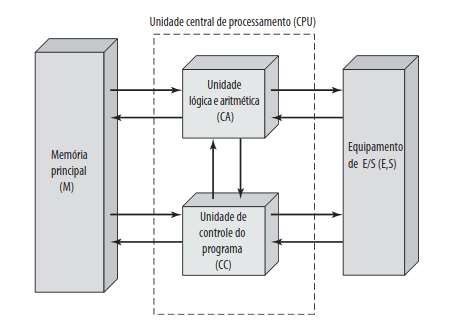
\includegraphics[width=\textwidth]{Figuras/computador-ias.png}

    \end{figure}

\end{frame}

\begin{frame}{A Estrutura Geral do Computador IAS}
    O computador IAS foi baseado na proposta inicial de von Neumann e serve como base para os computadores modernos. Ele consiste em quatro componentes fundamentais:

    \begin{itemize}
        \item \textbf{Memória Principal (M):} Responsável por armazenar tanto os dados quanto as instruções do programa.
        \item \textbf{Unidade Lógica e Aritmética (CA - Central Arithmetic):} Unidade especializada para realizar as operações aritméticas elementares e lógicas.
        \item \textbf{Unidade de Controle (CC - Central Control):} Órgão central que decodifica as instruções e sequencia a execução das operações.
        \item \textbf{Entrada e Saída (I/O - Input/Output):} Unidades encarregadas de realizar o contato com o meio exterior de gravação (R).
    \end{itemize}
\end{frame}

\begin{frame}{Estrutura da memória}

    \begin{figure}
        \centering

        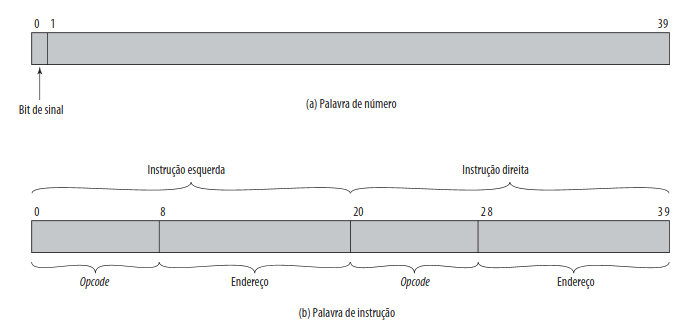
\includegraphics[width=\textwidth]{Figuras/memoria-ias.png}

    \end{figure}

\end{frame}

\begin{frame}{Formatos de Palavra no Computador IAS}
    A memória do IAS é organizada em 1.000 locais de armazenamento chamados \textbf{palavras} (\textit{words}), onde cada palavra possui \textbf{40 bits}.

    \begin{block}{Representação de Dados}
        \begin{itemize}
            \item \textbf{1 bit de sinal} seguido por um valor de \textbf{39 bits}.
        \end{itemize}
    \end{block}

    \begin{block}{Representação de Instruções}
        Uma palavra pode armazenar até \textbf{duas instruções de 20 bits} cada. Cada instrução é dividida em:
        \begin{itemize}
            \item \textbf{Código de Operação (Opcode):} 8 bits para especificar a operação.
            \item \textbf{Endereço:} 12 bits para apontar para uma das 1.000 palavras na memória.
        \end{itemize}
    \end{block}
\end{frame}

\begin{frame}{Computador IAS mais a fundo}

    \begin{figure}
        \centering

        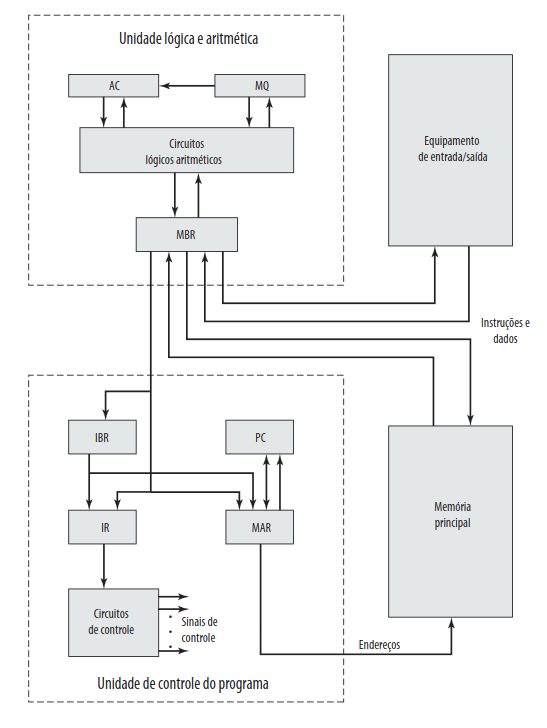
\includegraphics[width=0.55\textwidth]{Figuras/ias-expandido.png}

    \end{figure}

\end{frame}

\begin{frame}{Registradores da Unidade de Controle e ULA}
    Para buscar e executar as instruções passo a passo, o IAS utiliza um conjunto específico de registradores internos:

    \begin{itemize}
        \item \textbf{mBR (\textit{Memory Buffer Register}):} Contém a palavra que será enviada para a memória/E/S ou que acabou de ser recebida deles.
        \item \textbf{mAR (\textit{Memory Address Register}):} Especifica o endereço de memória da palavra que será lida ou gravada via mBR.
        \item \textbf{IR (\textit{Instruction Register}):} Guarda o opcode de 8 bits da instrução que está sendo executada no momento.
        \item \textbf{IBR (\textit{Instruction Buffer Register}):} Armazena temporariamente a segunda instrução da palavra para ser executada a seguir.
        \item \textbf{PC (\textit{Program Counter}):} Contém o endereço do próximo par de instruções que deve ser buscado na memória.
    \end{itemize}
\end{frame}

\begin{frame}{Registradores de Dados: AC e MQ}
    Para lidar com operandos e resultados da ALU, o IAS utiliza dois registradores especiais que trabalham em conjunto:

    \begin{itemize}
        \item \textbf{AC (Acumulador) e MQ (\textit{Multiplier Quotient}):} Empregados para manter temporariamente os operandos e os resultados das operações.
    \end{itemize}

    \begin{block}{Multiplicação de 40 bits $\rightarrow$ Resultado de 80 bits}
        Quando a ALU multiplica dois números de 40 bits, o resultado de 80 bits é dividido:
        \begin{itemize}
            \item \textbf{AC:} Armazena os 40 bits \textbf{mais significativos}.
            \item \textbf{MQ:} Armazena os 40 bits \textbf{menos significativos}.
        \end{itemize}
    \end{block}
\end{frame}

\begin{frame}{O Ciclo de Instrução do IAS}
    O funcionamento do IAS baseia-se na repetição contínua de um ciclo de instrução, dividido em dois subciclos principais:

    \begin{enumerate}
        \item \textbf{Ciclo de Busca (\textit{Fetch Cycle}):}
              \begin{itemize}
                  \item O \textit{opcode} da próxima instrução é carregado no \textbf{IR}.
                  \item A parte do endereço é carregada no \textbf{MAR}.
                  \item \textbf{Origem:} A instrução pode vir direto do \textbf{IBR} (se já estiver lá) ou ser buscada na memória via \textbf{MBR}.
              \end{itemize}
              \vspace{0.2cm}
        \item \textbf{Ciclo de Execução (\textit{Execute Cycle}):}
              \begin{itemize}
                  \item Com o \textit{opcode} no \textbf{IR}, o circuito de controle o interpreta.
                  \item Sinais de controle são enviados para mover dados ou ativar funções da ALU.
              \end{itemize}
    \end{enumerate}
\end{frame}

\begin{frame}{Por que a Indireção de Registradores?}
    No IAS, apenas o \textbf{MAR} especifica endereços de leitura/escrita e apenas o \textbf{MBR} serve como origem/destino de dados da memória.

    \begin{block}{Justificativa de Hardware}
        \begin{itemize}
            \item \textbf{Simplificação Eletrônica:} Reduz drasticamente a quantidade de caminhos de dados (\textit{data paths}) e multiplexadores necessários.
            \item \textbf{Controle Centralizado:} Facilita o projeto dos circuitos lógicos da Unidade de Controle.
        \end{itemize}
    \end{block}
\end{frame}

\begin{frame}{O Conjunto de Instruções do IAS (21 Instruções)}
    As 21 instruções do computador IAS podem ser agrupadas em 5 categorias funcionais:

    \begin{itemize}
        \item \textbf{Transferência de Dados:} Movem dados entre a memória e registradores da ALU, ou entre os próprios registradores da ALU.
        \item \textbf{Desvio Incondicional:} Altera a execução sequencial do programa, permitindo a criação de laços (\textit{loops}).
        \item \textbf{Desvio Condicional:} Permite tomar decisões no código baseando-se em condições (ex: se o valor for positivo).
        \item \textbf{Aritméticas:} Operações matemáticas executadas diretamente pelos circuitos da ALU.
        \item \textbf{Modificação de Endereço:} Permite que endereços sejam calculados na ALU e inseridos em instruções na memória, garantindo alta flexibilidade de endereçamento.
    \end{itemize}
\end{frame}

\begin{frame}{O Conjunto de Instruções do IAS (21 Instruções)}

    \begin{figure}
        \centering

        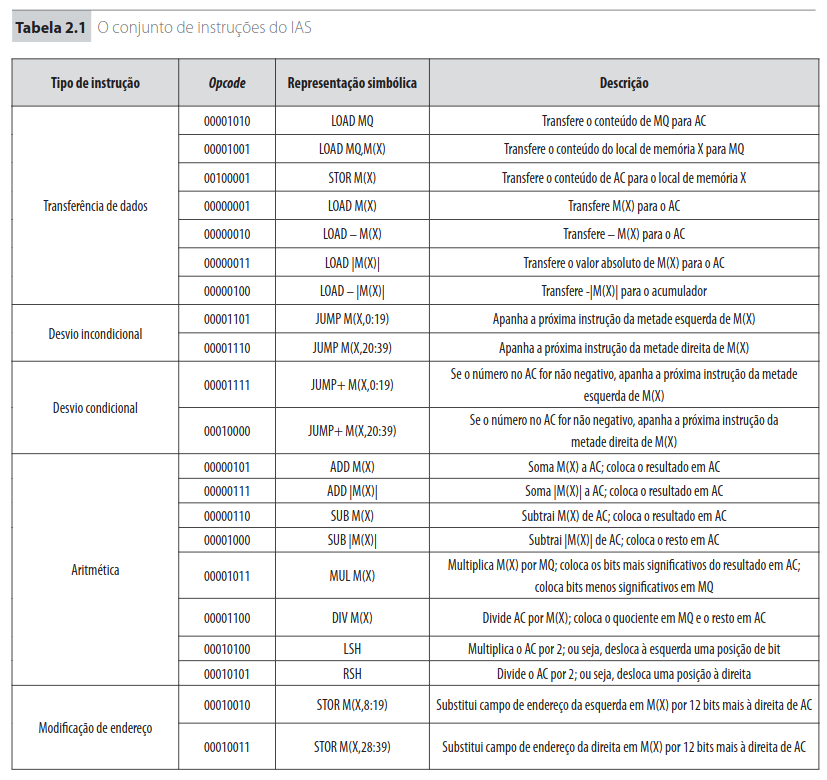
\includegraphics[width=0.79\textwidth]{Figuras/conjunto-instrucoes-ias.png}

    \end{figure}

\end{frame}